% Copyright 2004 by Till Tantau <tantau@users.sourceforge.net>.
%
% In principle, this file can be redistributed and/or modified under
% the terms of the GNU Public License, version 2.
%
% However, this file is supposed to be a template to be modified
% for your own needs. For this reason, if you use this file as a
% template and not specifically distribute it as part of a another
% package/program, I grant the extra permission to freely copy and
% modify this file as you see fit and even to delete this copyright
% notice. 

\documentclass{beamer}
\usepackage{menukeys}[os=win]
\usepackage{textcomp}
% There are many different themes available for Beamer. A comprehensive
% list with examples is given here:
% http://deic.uab.es/~iblanes/beamer_gallery/index_by_theme.html
% You can uncomment the themes below if you would like to use a different
% one:
%\usetheme{AnnArbor}
%\usetheme{Antibes}
%\usetheme{Bergen}
%\usetheme{Berkeley}
%\usetheme{Berlin}
%\usetheme{Boadilla}
%\usetheme{boxes}
%\usetheme{CambridgeUS}
%\usetheme{Copenhagen}
%\usetheme{Darmstadt}
%\usetheme{default}
%\usetheme{Frankfurt}
%\usetheme{Goettingen}
%\usetheme{Hannover}
%\usetheme{Ilmenau}
\usetheme{JuanLesPins}
%\usetheme{Luebeck}
%\usetheme{Madrid}
%\usetheme{Malmoe}
%\usetheme{Marburg}
%\usetheme{Montpellier}
%\usetheme{PaloAlto}
%\usetheme{Pittsburgh}
%\usetheme{Rochester}
%\usetheme{Singapore}
%\usetheme{Szeged}
%\usetheme{Warsaw}
\setbeamerfont{block body}{size=\small}
\title{KF5004 - \texttt{Ubuntu Server} Install and Networking}

% A subtitle is optional and this may be deleted
%\subtitle{(Using proximity detection)}

\author{Dr.~Neil~Eliot\inst{1} / Dr.~Alun~Moon\inst{1}}
% - Give the names in the same order as the appear in the paper.
% - Use the \inst{?} command only if the authors have different
%   affiliation.

%\renewcommand\appendixname{Appendix}

\institute[Northumbria University] % (optional, but mostly needed)
{
  \inst{1}
  Department of Computer and Information Sciences\\
  University of Northumbria
  % \and
  % \inst{2}
  % Department of Theoretical Philosophy\\
  % University of Elsewhere
}
% - Use the \inst command only if there are several affiliations.
% - Keep it simple, no one is interested in your street address.

\date{Session 2}
% - Either use conference name or its abbreviation.
% - Not really informative to the audience, more for people (including
%   yourself) who are reading the slides online

\subject{Introduction}
% This is only inserted into the PDF information catalog. Can be left
% out. 

% If you have a file called "university-logo-filename.xxx", where xxx
% is a graphic format that can be processed by latex or pdflatex,
% resp., then you can add a logo as follows:

% \pgfdeclareimage[height=0.5cm]{university-logo}{university-logo-filename}
% \logo{\pgfuseimage{university-logo}}

% Delete this, if you do not want the table of contents to pop up at
% the beginning of each subsection:
% \AtBeginSubsection[]
% {
%   \begin{frame}<beamer>{Outline}
%     \tableofcontents[currentsection,currentsubsection]
%   \end{frame}
% }

% Let's get started

\begin{document}

\begin{frame}
  \titlepage
\end{frame}

\begin{frame}{Introduction}
  \tableofcontents
  % You might wish to add the option [pausesections]
\end{frame}

% Section and subsections will appear in the presentation overview
% and table of contents.
\section{Version}
\begin{frame}{Which version do we use?}
  \begin{figure}
    \begin{center}
      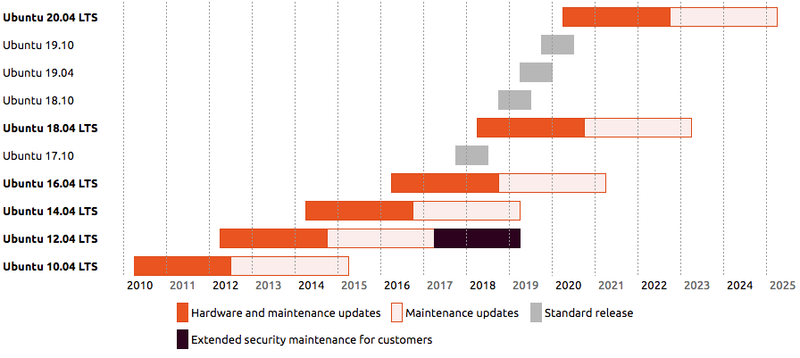
\includegraphics[width=1\linewidth]{Version.png}
    \end{center}
  \end{figure}
\end{frame}

\begin{frame}{Which version do we use?}
  \begin{center}
    \LARGE This year we will be using:-\\
    \Huge \texttt{18.04 LTS}
  \end{center}
\end{frame}

\section{Installation}
\subsection{General}
\begin{frame}{Headless}
  \begin{itemize}
    \item Server machines (*nix) are generally in `Headless' mode.
    \begin{itemize}
      \item No Monitor.
      \item No Keyboard.
      \end{itemize}
    \item Located in a climate controlled server room.
    \item Most maintenance is carried out remotely via a secure terminal login.
      \begin{itemize}
        \item \texttt{Putty} (\texttt{Windows/Linux})
        \item \texttt{ssh} (\texttt{Windows/Linux})
          \begin{itemize}
            \item \texttt{e.g. \$ssh student@192.168.150.99}
            \item \texttt{e.g. C:\textbackslash\textgreater ssh student@192.168.150.99}
          \end{itemize}
        \end{itemize}
  \end{itemize}
\end{frame}

\begin{frame}{Installer}
  \begin{itemize}
    \item Ubuntu Server \texttt{ISO} can be downloaded from:
      \begin{itemize}
        \item \texttt{https://www.ubuntu.com}
      \end{itemize}
    \item There is also an ISO located on the Lab NAS drive:
      \begin{itemize}
        \item \texttt{\textbackslash\textbackslash NAS3}
        \item \texttt{\textbackslash\textbackslash NAS3.offcampusnetwork.co.uk}
      \end{itemize}
  \end{itemize}
\end{frame}

\begin{frame}{Install \texttt{Ubuntu Server}}
  \begin{itemize}
    \item Select all the options that give you a \texttt{UK English} keyboard.
    \item Select default disc configuration.
    \item Set machine name to your \texttt{`<student id>'}
      \begin{itemize}
        \item e.g. \texttt{A12345678}
        \item Later in the module you should use names that relate to the service the machine will support e.g. \texttt{DNS1}
      \end{itemize}
    \item The above process will create:-
      \begin{itemize}
        \item Minimal install with no unnecessary packages.
        \item No graphical interface (\texttt{GUI}).
      \end{itemize}
  \end{itemize}
\end{frame}

\begin{frame}{Install \texttt{Ubuntu Server}}
  \begin{itemize}
    \item On completion of the installation you will only be able to login via the machines console.
    \item To become a headless server remote access software must be installed.
      \begin{itemize}
        \item \texttt{ssh} or \texttt{telnet}
      \end{itemize}
  \end{itemize}
  \begin{block}{NOTE}
    Installation of remote access services will be covered later. Also there are security issues with \texttt{telnet}. 
  \end{block}
\end{frame}

\subsection{VMWare}
\begin{frame}{Install \texttt{Ubuntu Server} (\texttt{VMWare})}
  \begin{center}
    \begin{figure}
      \begin{overprint}
        \setlength{\fboxsep}{0pt}%
        \setlength{\fboxrule}{0.5pt}%
        \onslide<1>\centering\fbox{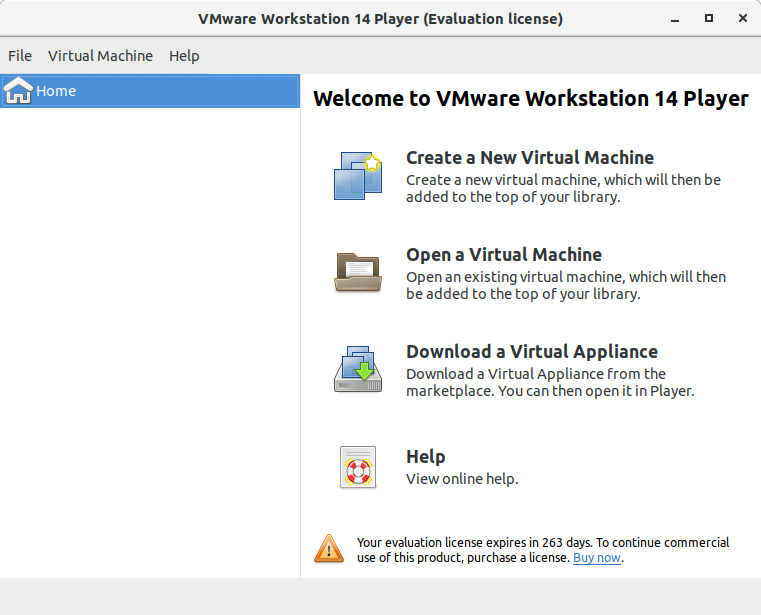
\includegraphics[width=.7\textwidth]{VMWare1.png}}
        \onslide<2>\centering\fbox{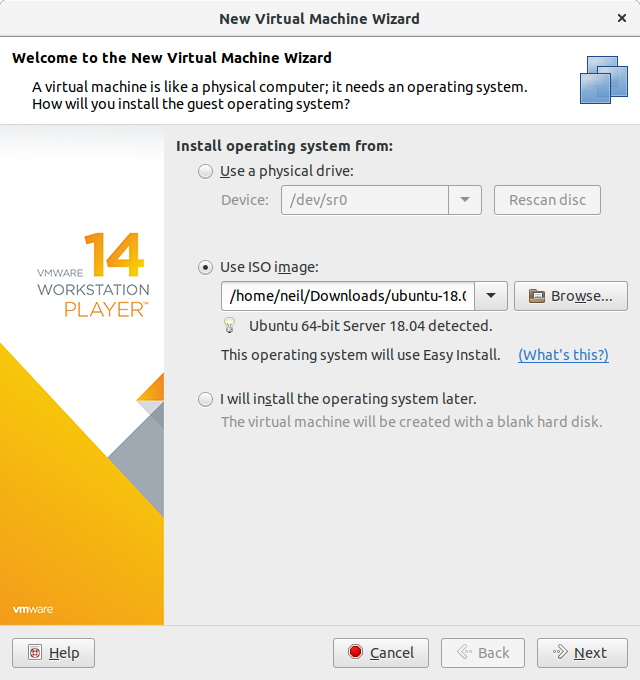
\includegraphics[width=.6\textwidth]{VMWare2.png}}
        \onslide<3>\centering\fbox{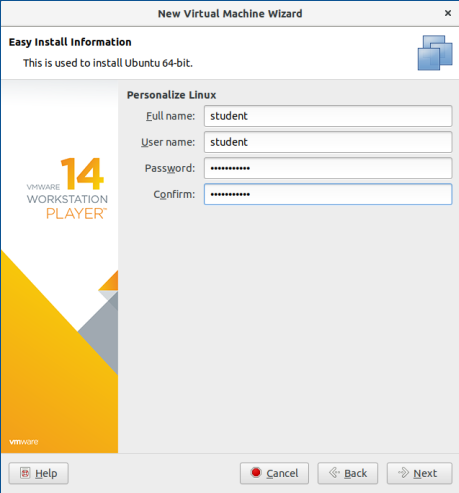
\includegraphics[width=.6\textwidth]{VMWare3.png}}
        \onslide<4>\centering\fbox{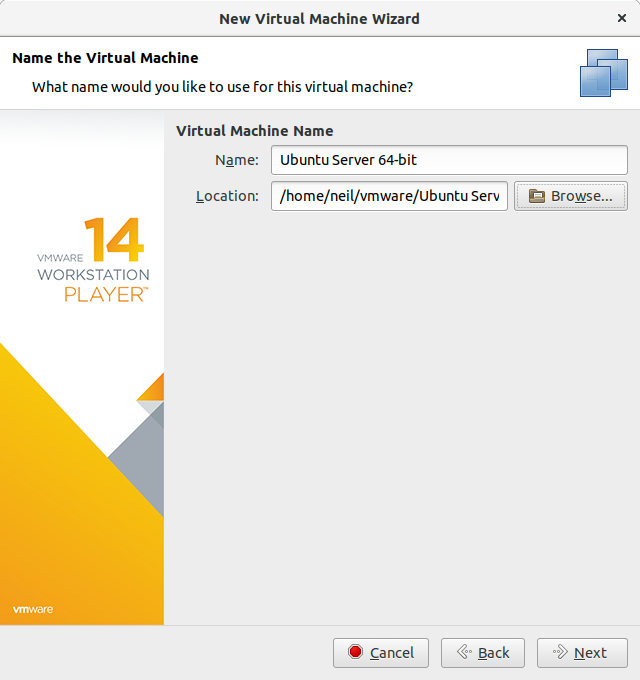
\includegraphics[width=.6\textwidth]{VMWare4.png}}
        \onslide<5>\centering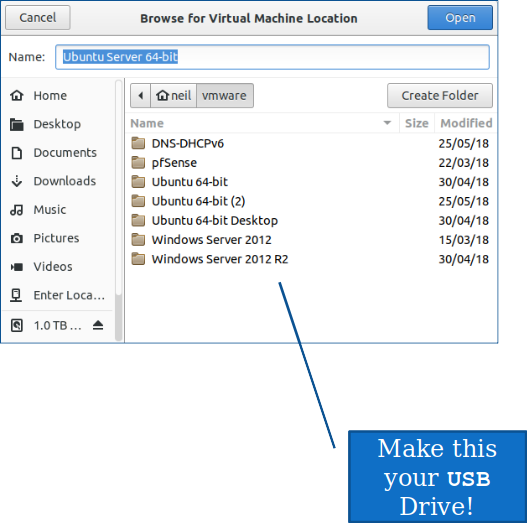
\includegraphics[width=.6\textwidth]{VMWare5.png}
        \onslide<6>\centering\fbox{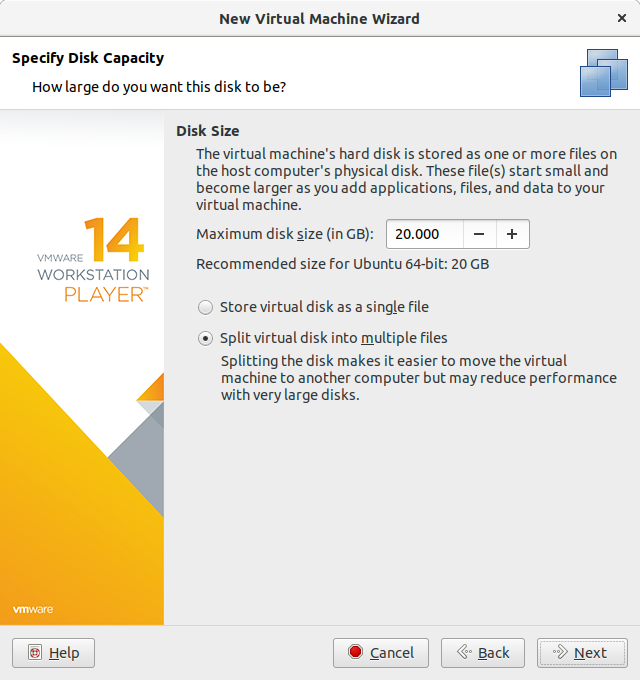
\includegraphics[width=.6\textwidth]{VMWare6.png}}
        \onslide<7>\centering\fbox{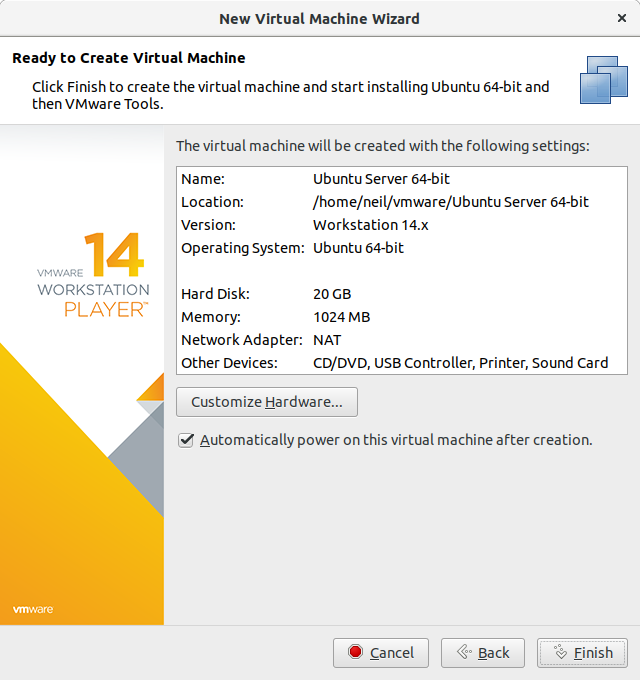
\includegraphics[width=.6\textwidth]{VMWare7.png}}
        \onslide<8>\centering\fbox{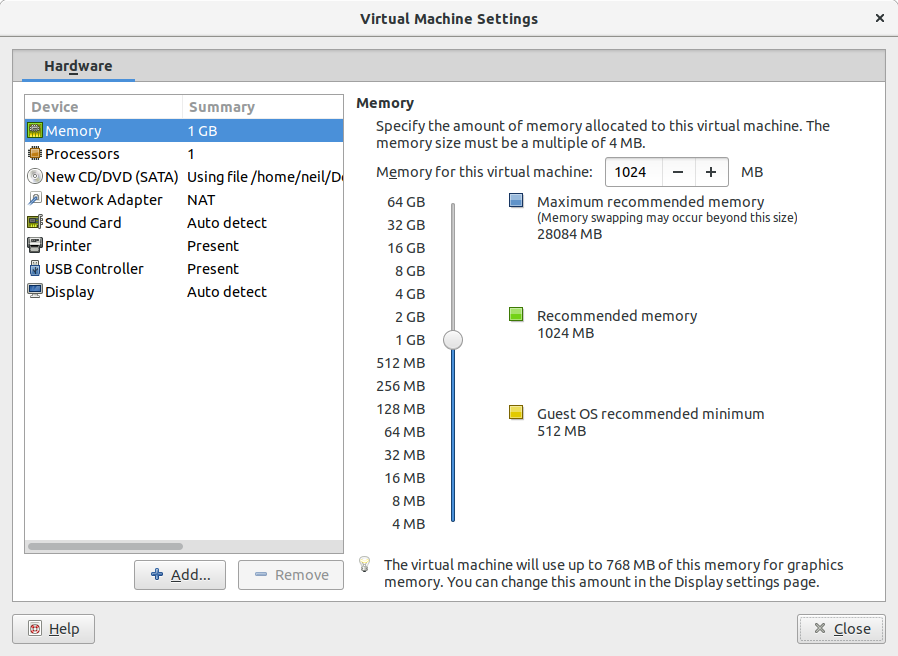
\includegraphics[width=.6\textwidth]{VMWare8.png}}
        \onslide<9>\centering\fbox{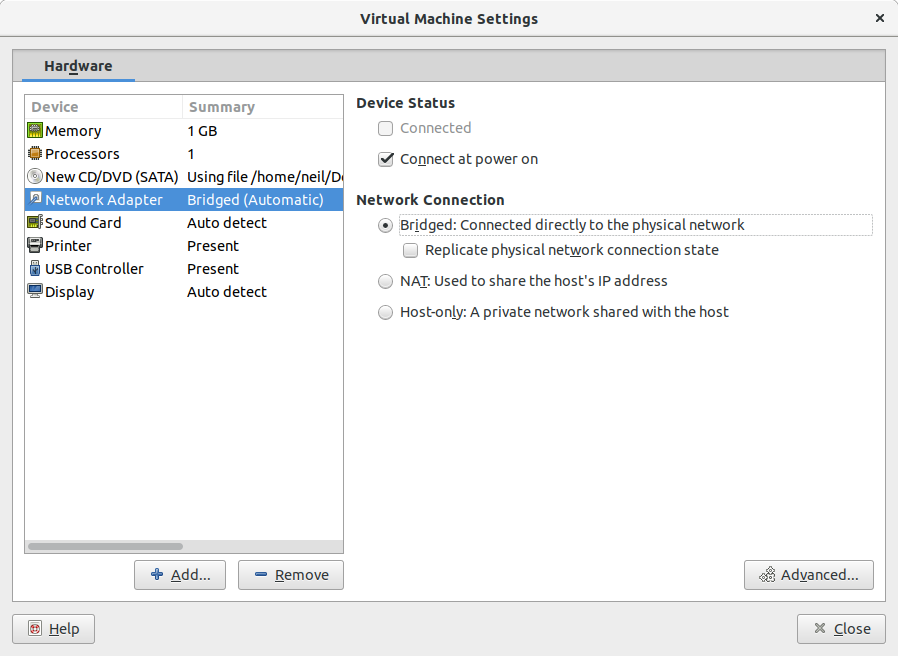
\includegraphics[width=.6\textwidth]{VMWare9.png}}
        \onslide<10>\centering\fbox{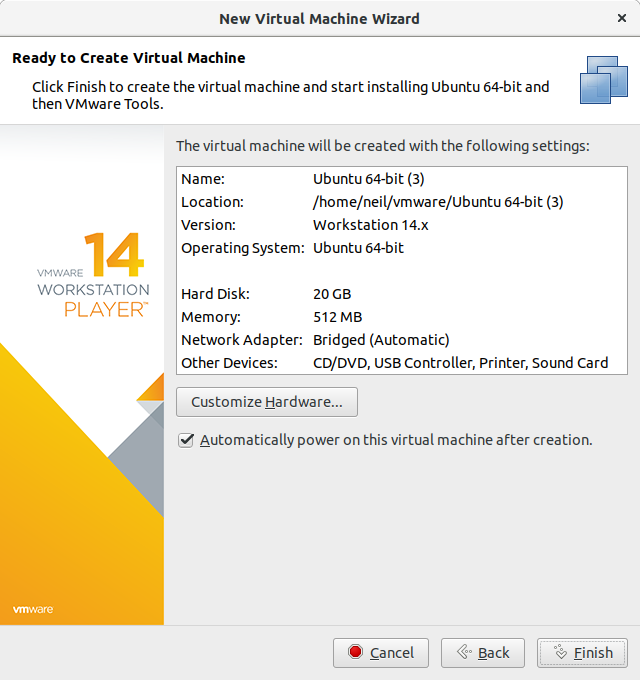
\includegraphics[width=.6\textwidth]{VMWare10.png}}
      \end{overprint}      
    \end{figure}
  \end{center}
\end{frame}

\subsection{Ubuntu}
\begin{frame}{Install \texttt{Ubuntu Server} (\texttt{Ubuntu})}
  \begin{figure}
    \begin{overprint}
      \setlength{\fboxsep}{0pt}%
      \setlength{\fboxrule}{0.5pt}%
      \onslide<1>\centering\fbox{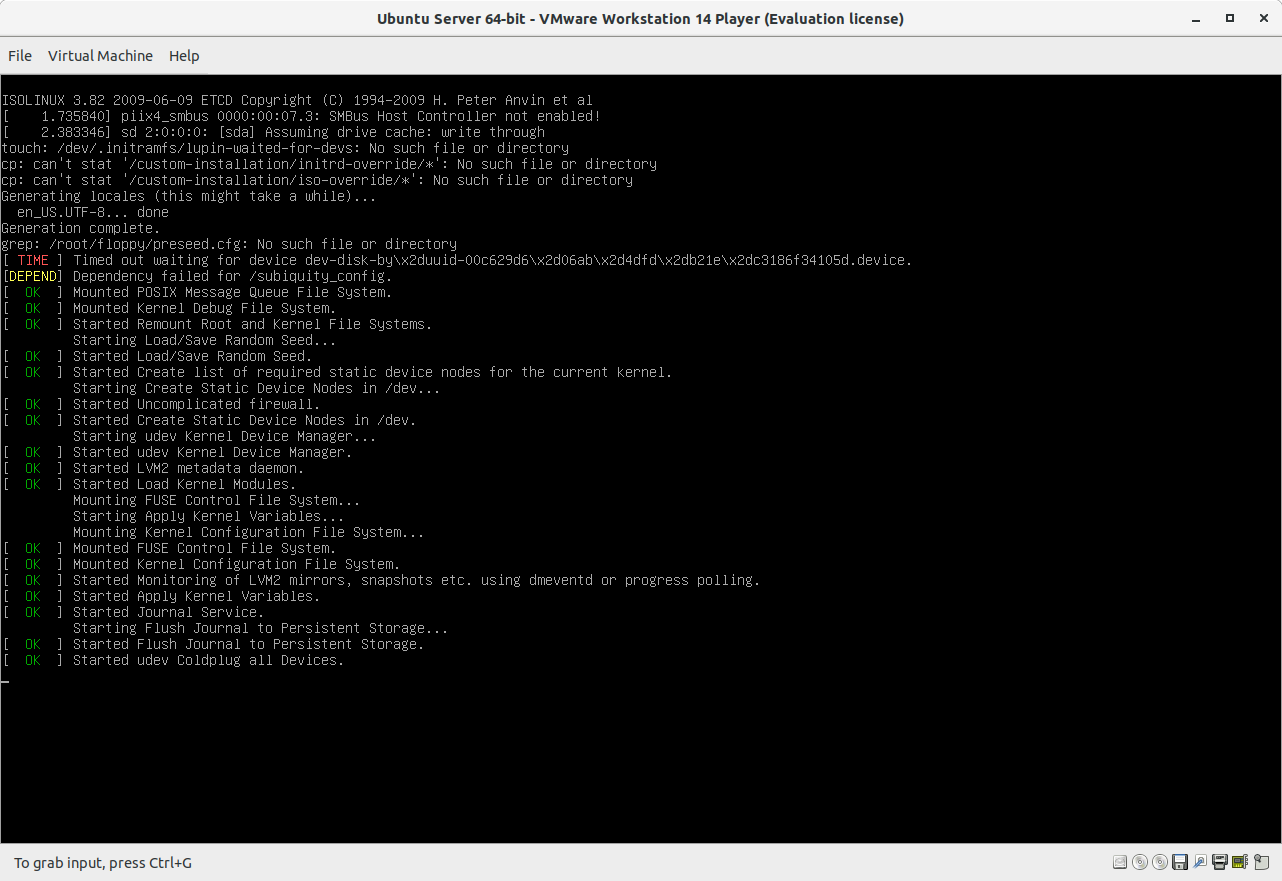
\includegraphics[width=.8\textwidth]{Ubuntu1.png}}
      \onslide<2>\centering\fbox{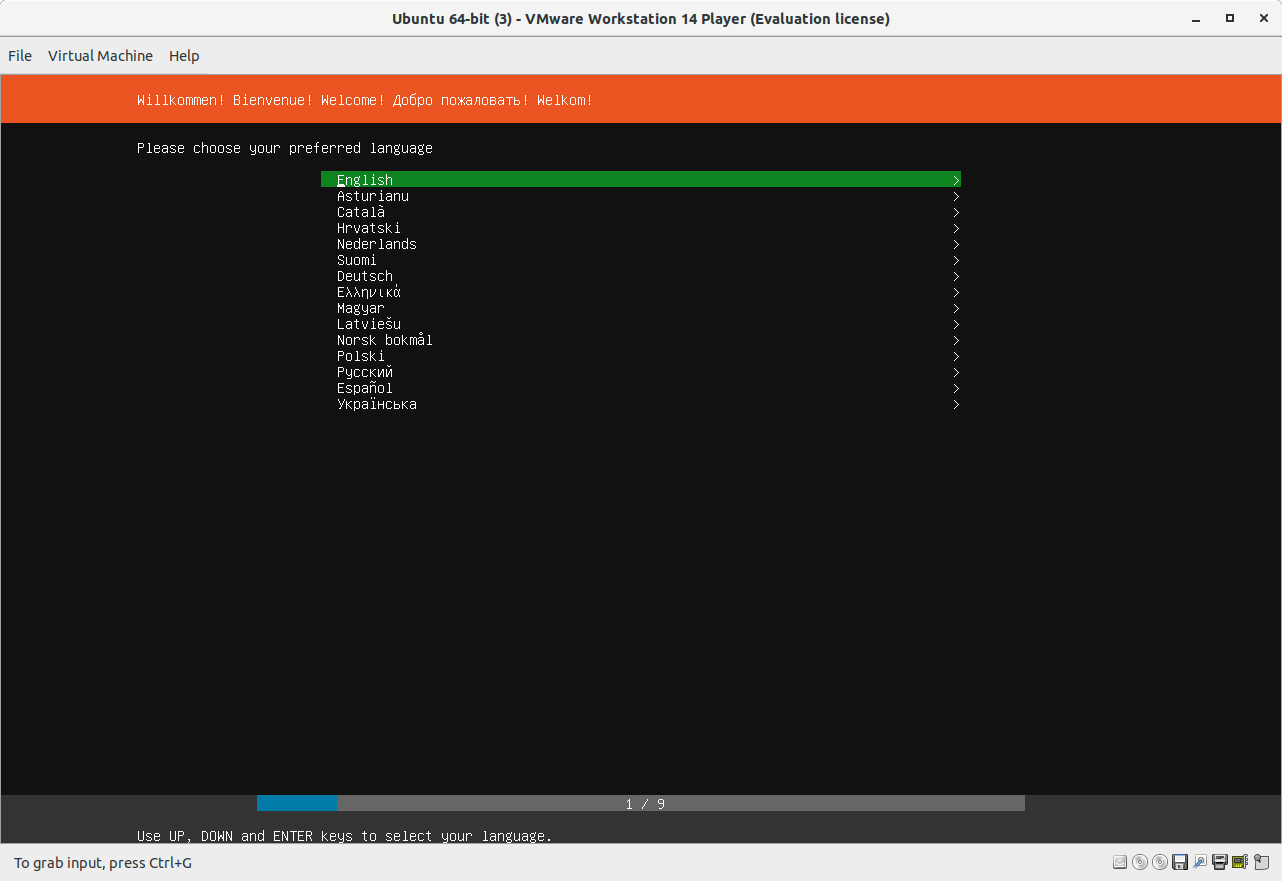
\includegraphics[width=.8\textwidth]{Ubuntu2.png}}
      \onslide<3>\centering\fbox{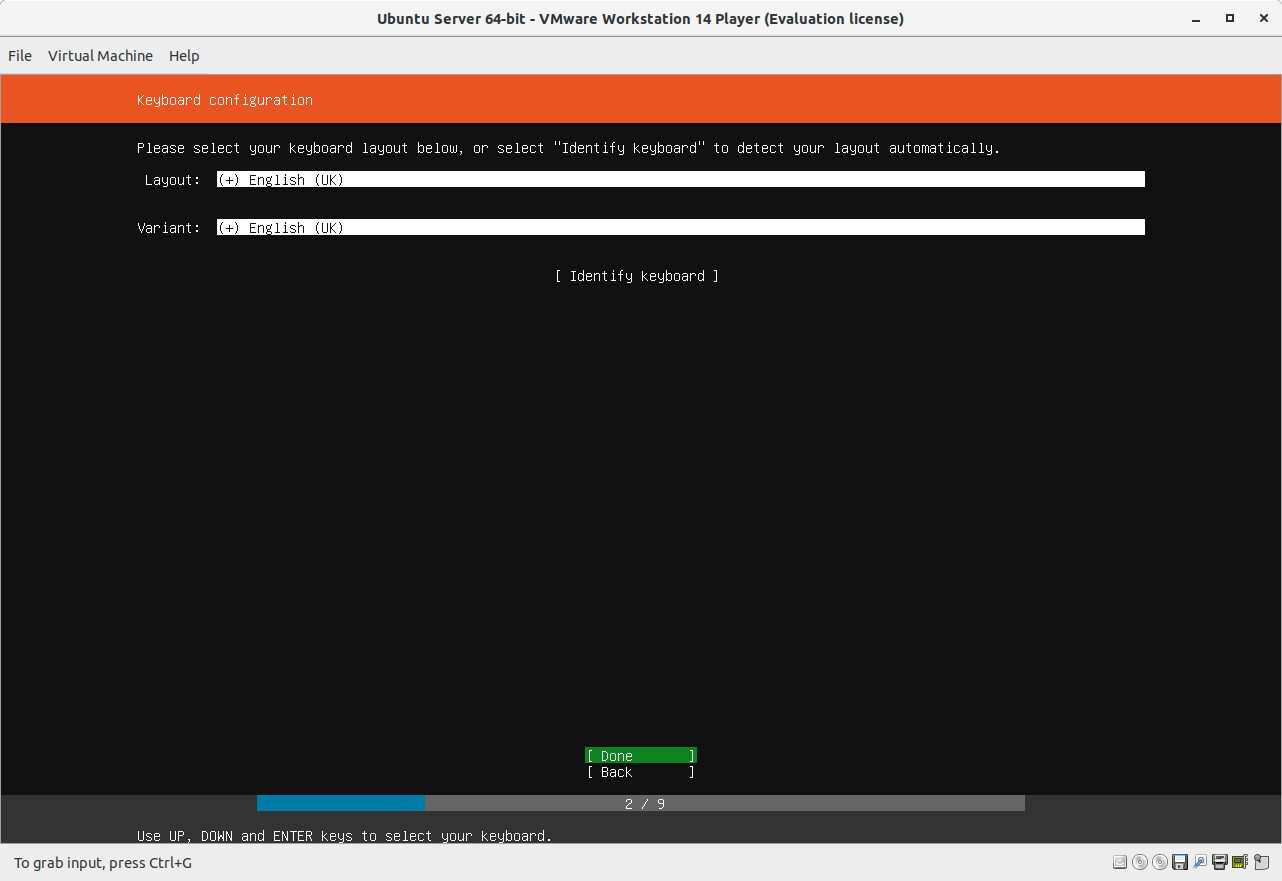
\includegraphics[width=.8\textwidth]{Ubuntu3.png}}
      \onslide<4>\centering\fbox{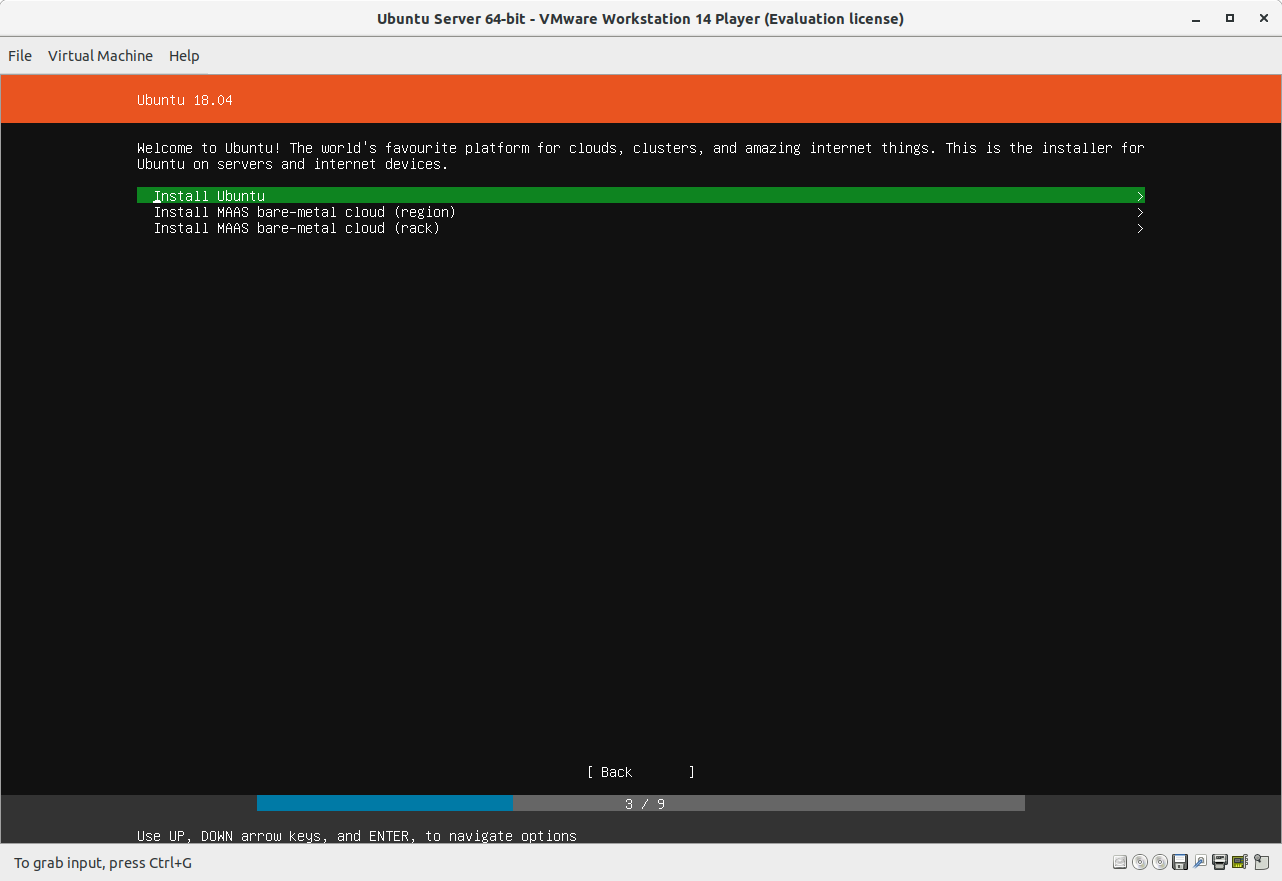
\includegraphics[width=.8\textwidth]{Ubuntu4.png}}
      \onslide<5>\centering\fbox{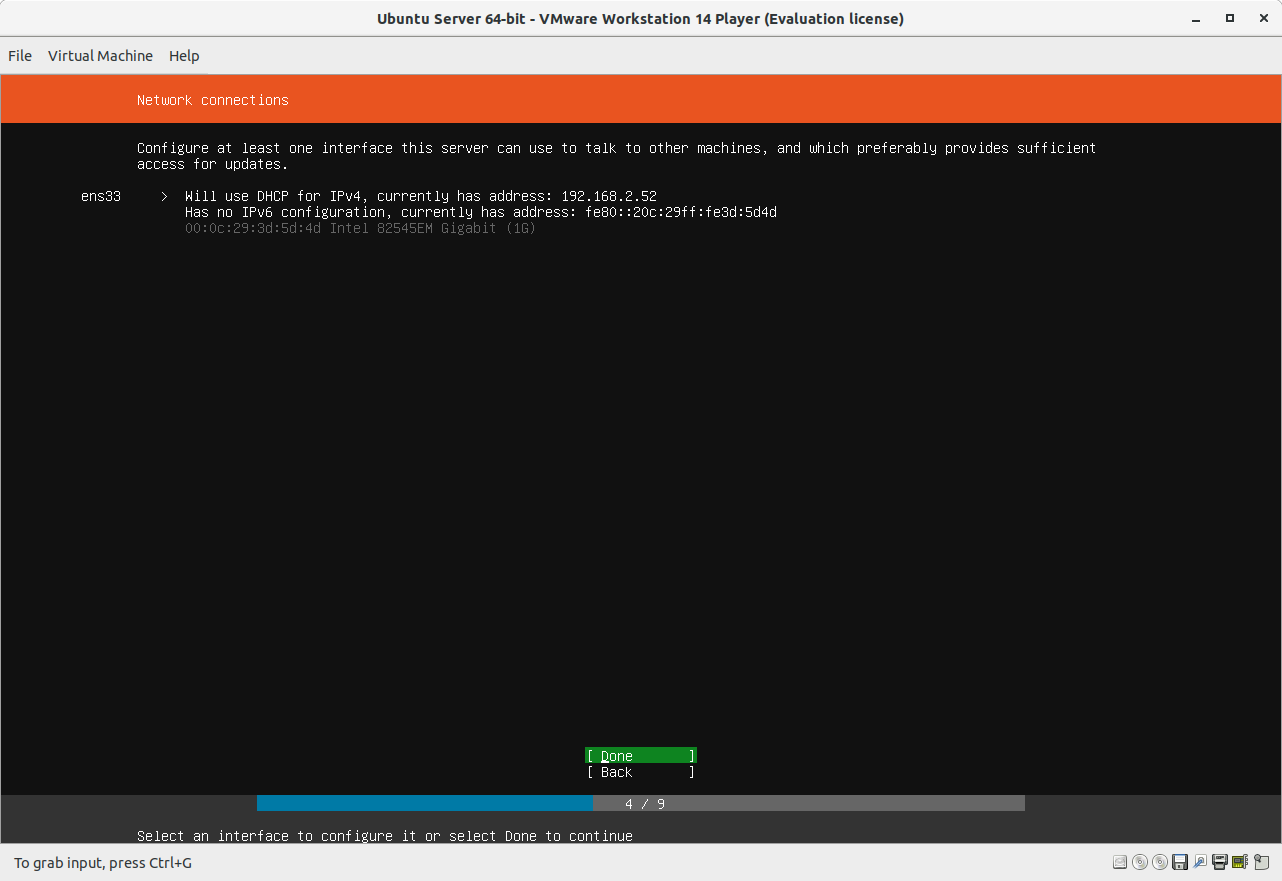
\includegraphics[width=.8\textwidth]{Ubuntu5.png}}
      \onslide<6>\centering\fbox{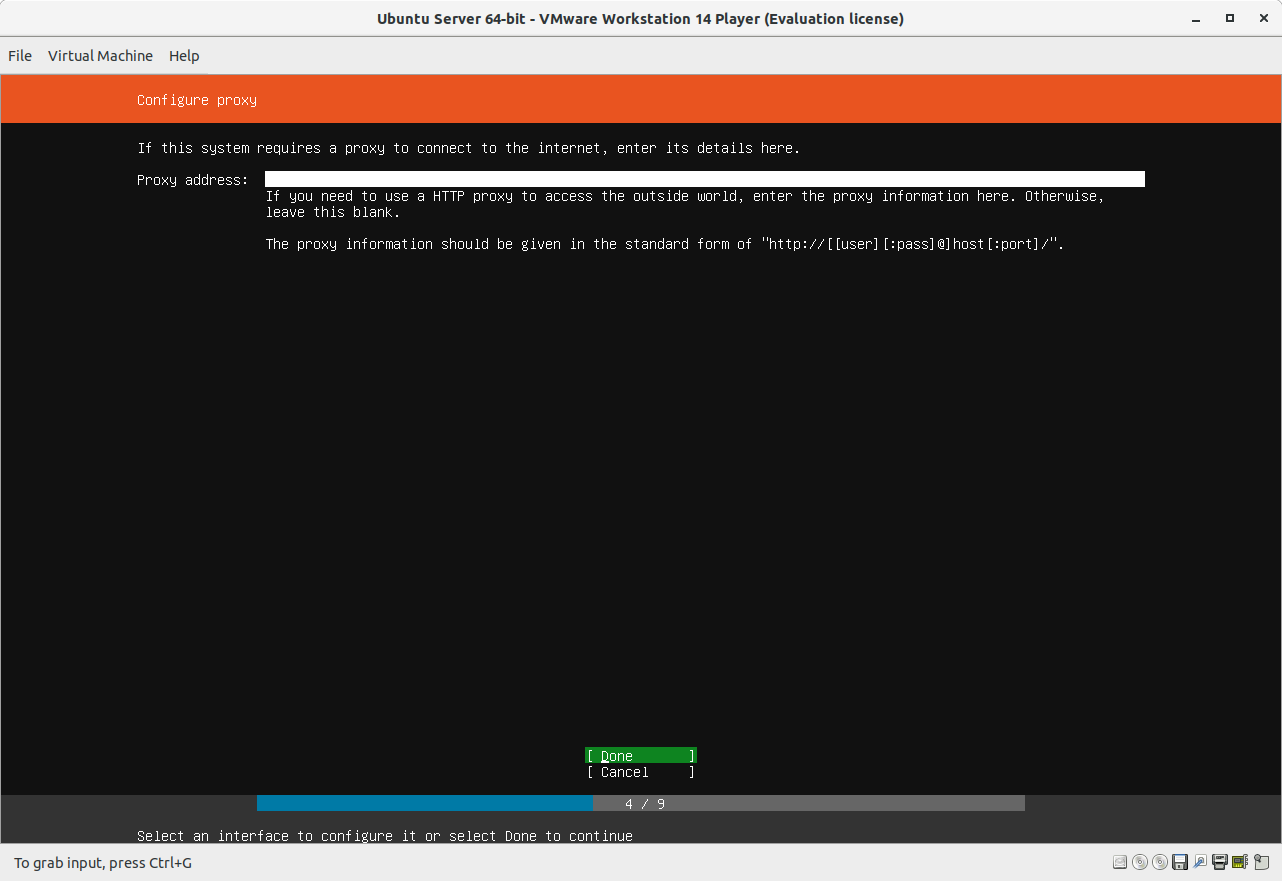
\includegraphics[width=.8\textwidth]{Ubuntu6.png}}
      \onslide<7>\centering\fbox{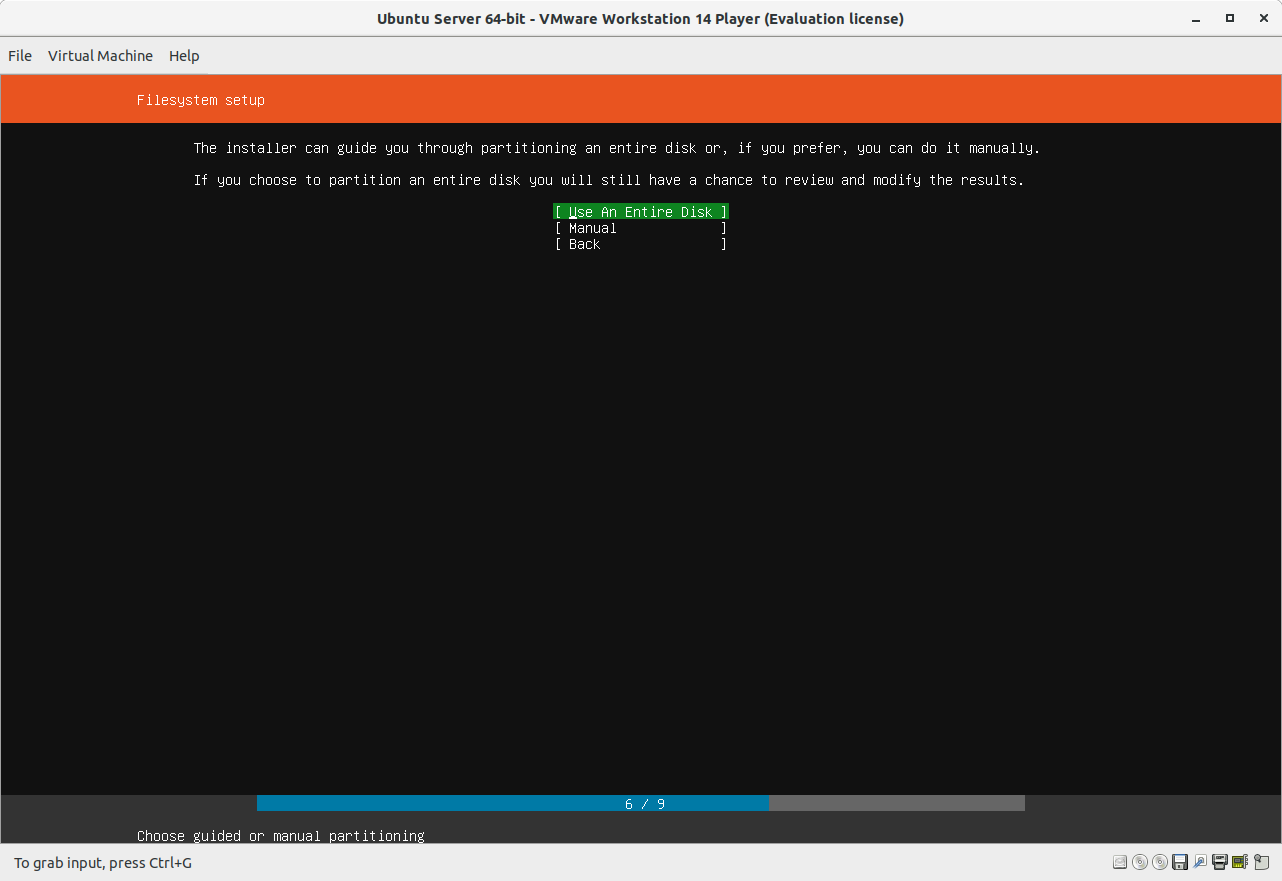
\includegraphics[width=.8\textwidth]{Ubuntu7.png}}
      \onslide<8>\centering\fbox{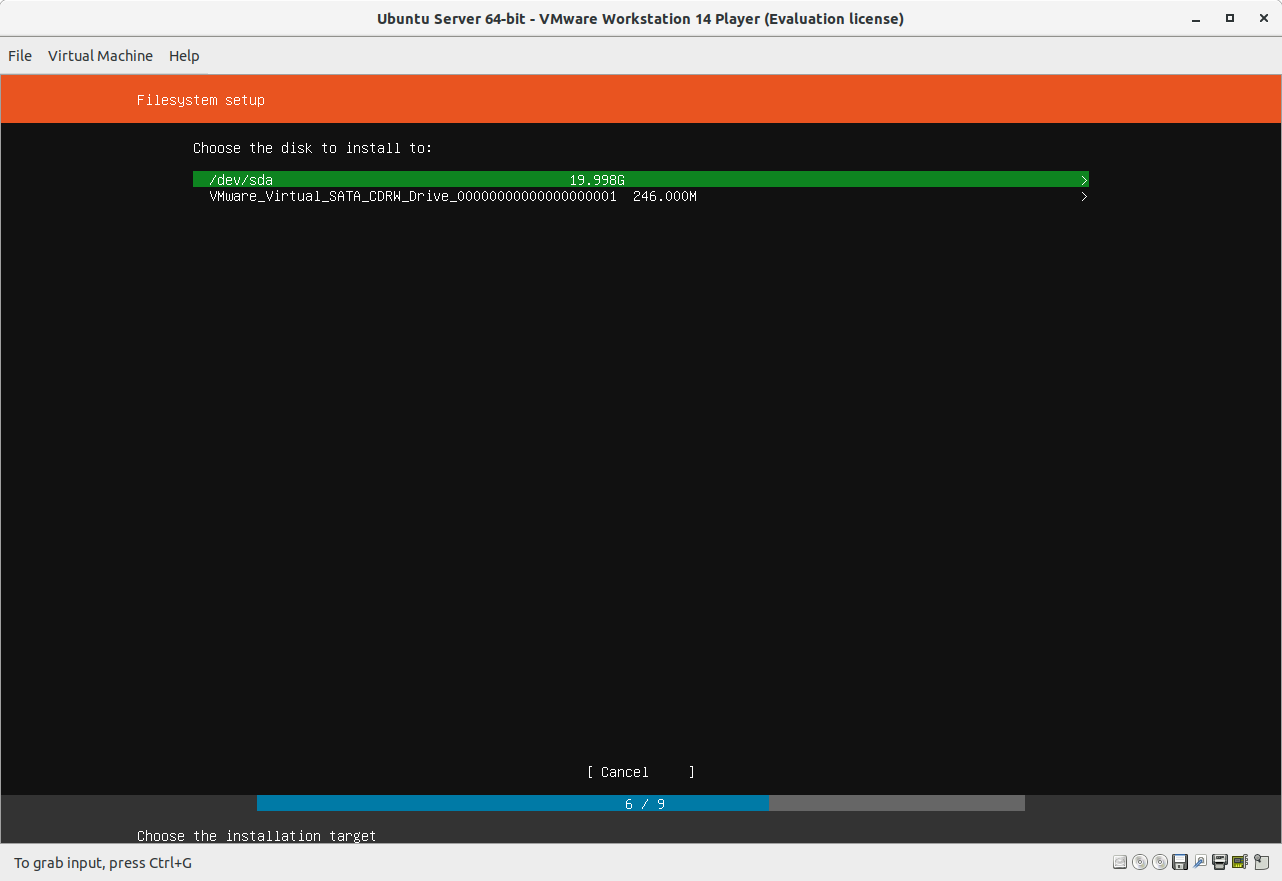
\includegraphics[width=.8\textwidth]{Ubuntu8.png}}
      \onslide<9>\centering\fbox{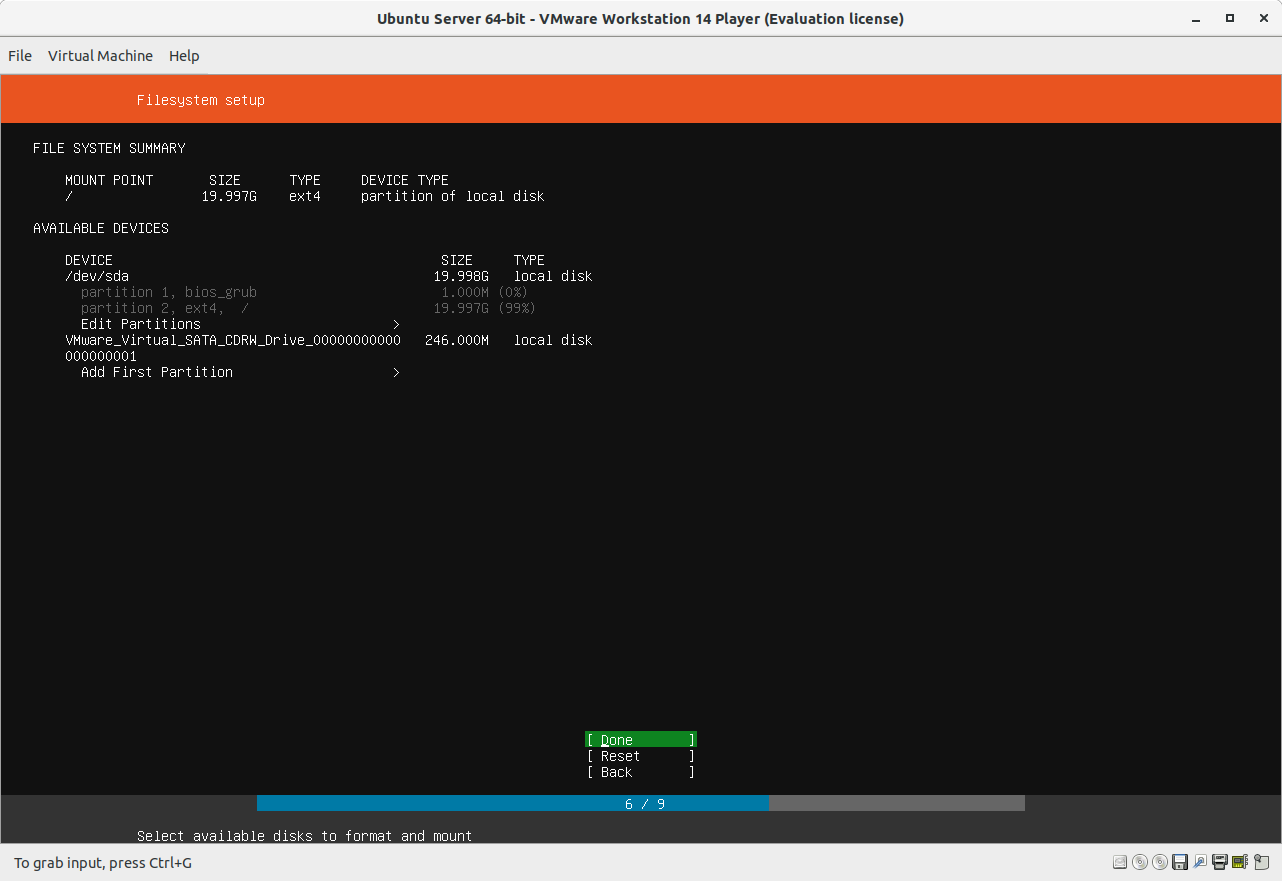
\includegraphics[width=.8\textwidth]{Ubuntu9.png}}
      \onslide<10>\centering\fbox{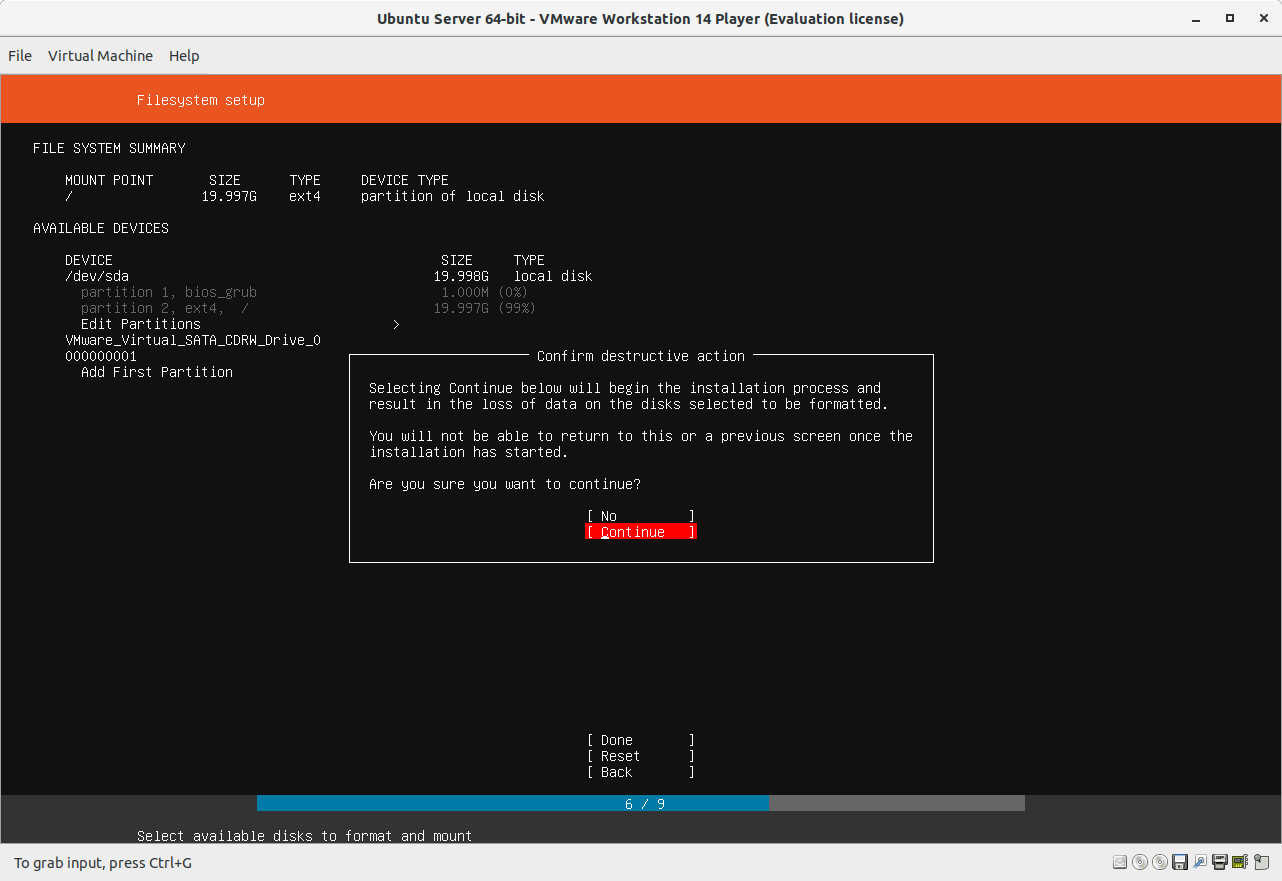
\includegraphics[width=.8\textwidth]{Ubuntu10.png}}
      \onslide<11>\centering\fbox{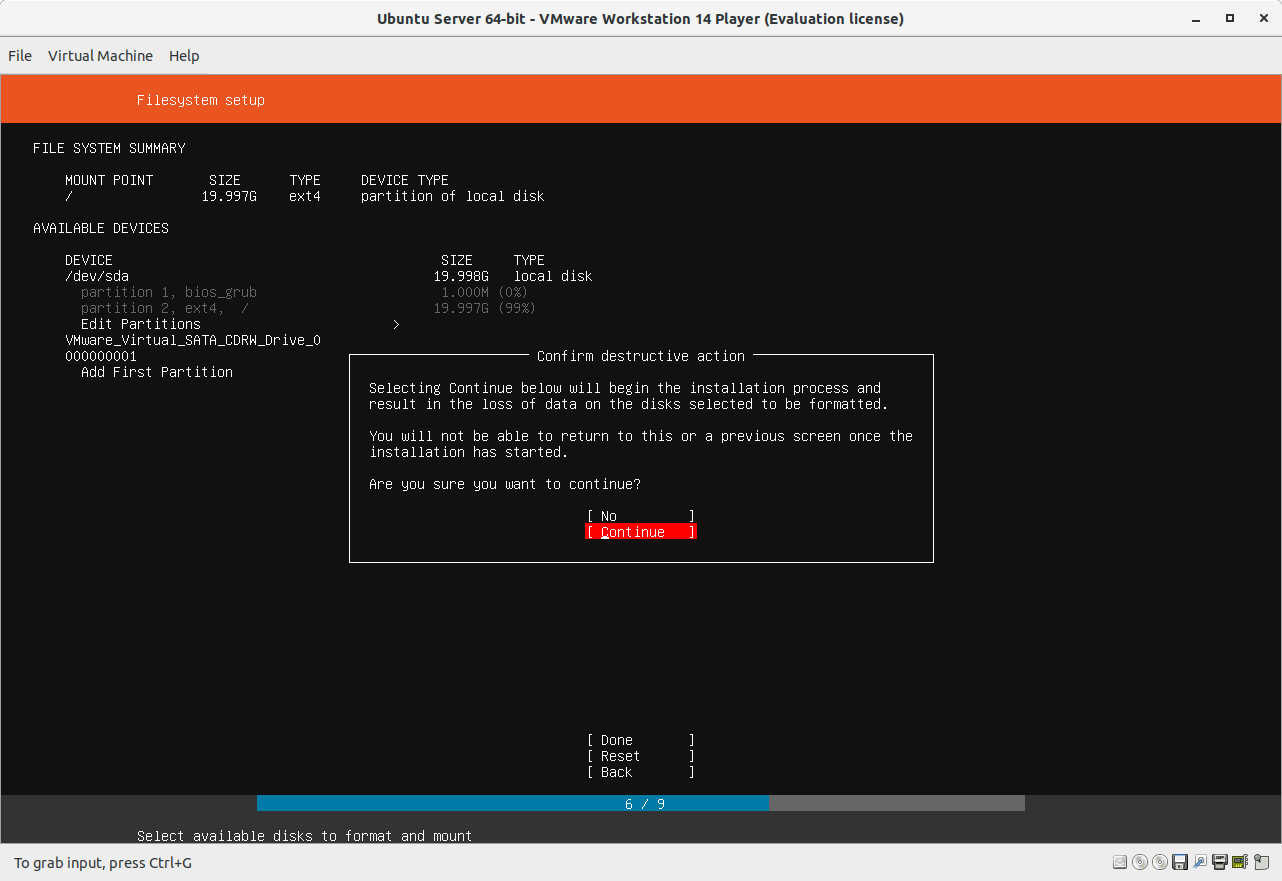
\includegraphics[width=.8\textwidth]{Ubuntu11.png}}
      \onslide<12>\centering\fbox{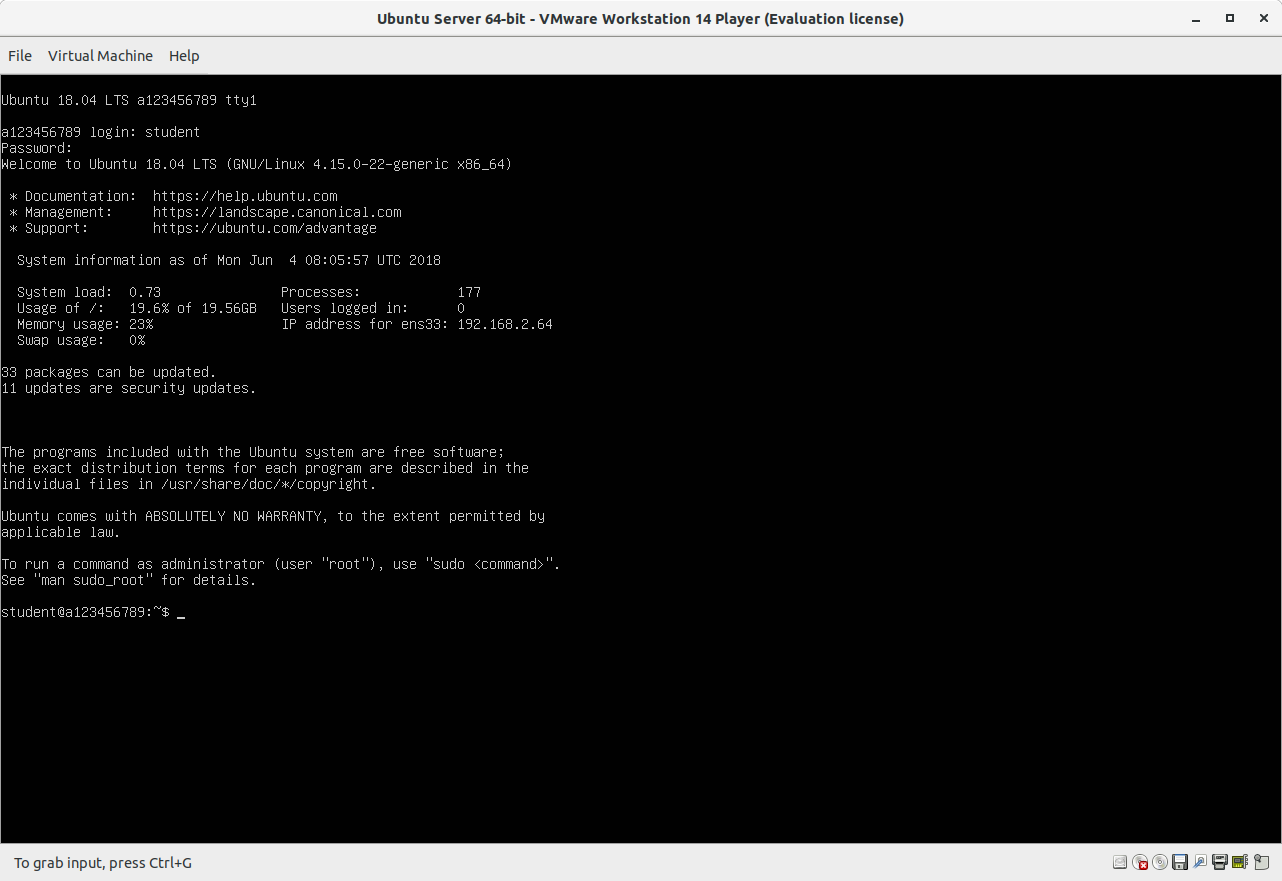
\includegraphics[width=.8\textwidth]{Ubuntu12.png}}
    \end{overprint}
  \end{figure}
\end{frame}

\section{Post Install}
\subsection{Updating}
\begin{frame}{Update your \texttt{Ubuntu Server} software}
  \begin{itemize}
    \item The server \texttt{OS} may need updated. This will require the repository database to be updated before the upgrade is actioned.
      \begin{itemize}
        \item Update the repository database.
          \begin{itemize}
            \item \texttt{sudo apt-get update}
          \end{itemize}
        \item Update the software.
          \begin{itemize}
            \item \texttt{sudo apt-get upgrade}
          \end{itemize}
      \end{itemize}
  \end{itemize}
  \begin{block}{NOTE}
    This should be done on a regular basis to ensure bugs and vulnerabilities are patched (weekly or adhoc?). 
  \end{block}
\end{frame}

\subsection{Essential Packages}
\begin{frame}{Remote access (Headless server)}
  \begin{itemize}
    \item Once the remote software is added you can connect via the network rather than the console.
      \begin{itemize}
        \item To install \texttt{ssh} (\texttt{S}ecure \texttt{SH}ell)
          \begin{itemize}
            \item \texttt{sudo apt-get install openssh-server}
          \end{itemize}
        \item To install \texttt{telnet}
          \begin{itemize}
            \item \texttt{sudo apt-get install telnetd}
          \end{itemize}
      \end{itemize}
  \end{itemize}
\end{frame}

\begin{frame}{Remote access (Headless server)}
  \begin{itemize}
    \item To get the IP address of your machine use the command.
      \begin{itemize}
        \item \texttt{\$ip a}
      \end{itemize}
  \end{itemize}
  \begin{figure}
    \begin{center}
      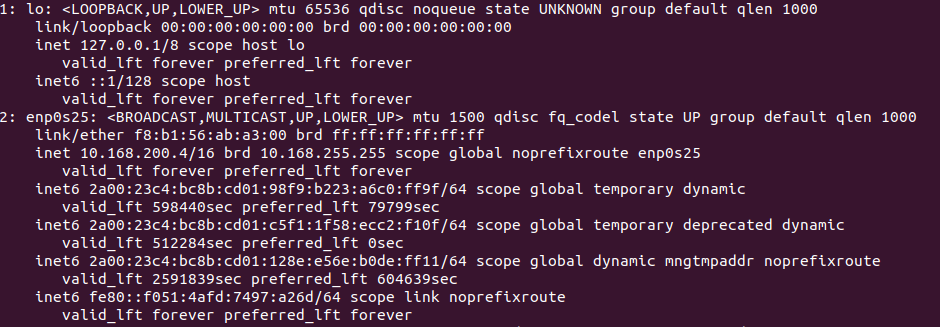
\includegraphics[width=1\linewidth]{ip.png}
    \end{center}
  \end{figure}
\end{frame}

\begin{frame}{Remote access (Headless server)}
  \begin{itemize}
    \item Putty settings.
      \begin{itemize}
        \item \texttt{ip}
        \item Connection type (protocol)
      \end{itemize}
  \end{itemize}
  \begin{figure}
    \begin{center}
      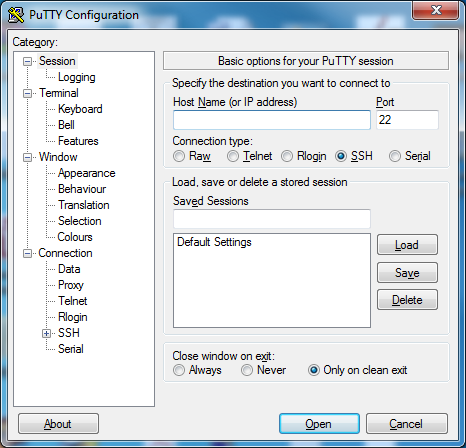
\includegraphics[width=0.5\linewidth]{Putty1.png}
    \end{center}
  \end{figure}
\end{frame}

\begin{frame}{Remote access (Headless server)}
  \begin{itemize}
    \item Check your connection by looking at the running process from the console.
      \begin{itemize}
        \item \texttt{\$ps -ef | grep sshd}
      \end{itemize}
  \end{itemize}
  \begin{figure}
    \begin{center}
      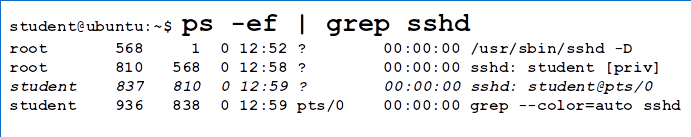
\includegraphics[width=1\linewidth]{ps.png}
    \end{center}
  \end{figure}
  \begin{itemize}
      \item \texttt{ssh} is a secure method of connecting to the server if you use \texttt{telnet} all commands are sent as plain text over the Ethernet connection and can be intercepted.
  \end{itemize}
\end{frame}
% Placing a * after \section means it will not show in the
% outline or table of contents.  

\begin{frame}{Connectivity Testing}
  \begin{itemize}
    \item By default \texttt{ping} and other simple tools are included but you may want to install \texttt{traceroute}. 
      \begin{itemize}
        \item \texttt{\$sudo apt-get install traceroute}
      \end{itemize}
    \item \texttt{traceroute} checks traffic routing from source to destination.
      \begin{itemize}
        \item \texttt{\$traceroute www.google.com}
      \end{itemize}
  \end{itemize}
\end{frame}

\begin{frame}{\texttt{IP} Addressing considerations}
   \begin{itemize}
     \item Internet services are generally fixed in nature with a specific function. 
     \item Network services are vital to normal operations an therefore need to be implemented with \textbf{Redundancy} and \textbf{Fault Tolerance} in mind.
     \item Generally they have a static \texttt{IP} address to maintain access to the service (Network servers should, as far as is possible, not be dependant on other services e.g. \texttt{DHCP}) and are referenced by their \texttt{IP} address.
   \end{itemize}
   \begin{block}{NOTE}
     Check your desktop machine's config for the \texttt{gateway} and \texttt{name servers}. They are  all specified as \texttt{IP} Addresses!
   \end{block}
\end{frame}

\begin{frame}{Static \texttt{IP} Addressing}
  \begin{itemize}
    \item Almost all configurations in a Linux server are performed using text based configuration files.
    \item Reloading configurations is a simple matter of restarting the service/daemon (program).
    \item Generally they have a static \texttt{IP} address to maintain access to the service (Network servers should, as far as is possible, not be dependant on other services e.g. \texttt{DHCP}) and are referenced by their \texttt{IP} address.
  \end{itemize}
\end{frame}

\begin{frame}{Static \texttt{IP} Addressing}
  \begin{itemize}
    \item The location of the network config files on a \texttt{18.04 Ubuntu server} are:-
    \begin{itemize}
      \item \texttt{/etc/netplan}
    \end{itemize} 
  \end{itemize}
  \begin{block}{NOTE}
    If netplan is disabled.
    \begin{itemize}
      \item \texttt{/etc/network/interfaces}
      \item \texttt{/etc/resolv.conf}
      \item \texttt{/etc/hosts}
    \end{itemize} 
  \end{block}
\end{frame}

\begin{frame}{Static \texttt{IP} Addressing}
  \begin{itemize}
    \item \texttt{netplan} files are in YAML format.
    \begin{itemize}
      \item \texttt{/etc/netplan}
    \end{itemize} 
  \end{itemize}
  \begin{block}{CITATION}
    Yaml.org. (2018). \textit{The Official YAML Web Site.} [online] Available at: \texttt{http://yaml.org/} [Accessed 8 July. 2019].
  \end{block}
\end{frame}

\begin{frame}{Static \texttt{IP} Addressing}
  \begin{itemize}
    \item There can be several configuration files that are parsed sequentially (based on initial numeric).
    \item File location:-
    \begin{itemize}
      \item \texttt{/etc/netplan}
    \end{itemize} 
    \item The files are in \texttt{YAML} format.
    \item The default network configuration file is :-
    \begin{itemize}
      \item \texttt{50-cloud-init.yaml}
    \end{itemize} 
  \end{itemize}
\end{frame}

\begin{frame}{Static \texttt{IP} Addressing}
  \begin{itemize}
    \item Default configuration:-
  \end{itemize}
    \begin{center}
      \begin{minipage}{8cm}
        \begin{block}{}
          \texttt{\# This file describes ...\\
          \# For more information, see netplan(5).\\
          ~~network:\\
          ~~version: 2\\
          ~~renderer: networkd\\
          ~~ethernets:\\
          ~~~~ens33:\\
          ~~~~~~dhcp4: yes\\
          ~~~~~~dhcp6: yes}
        \end{block}
      \end{minipage}
    \end{center}
\end{frame}

\begin{frame}{Static \texttt{IP} Addressing}
  \begin{itemize}
    \item Any changes made to the file are applied using the netplan command:-
    \begin{itemize}
      \item \texttt{\$sudo netplan apply}
    \end{itemize}
  \end{itemize}
\end{frame}

\begin{frame}{Static \texttt{IP} Addressing}
  \begin{itemize}
    \item For a static address modify the default configuration rather than created another otherwise you will have multiple IP addresses allocated.
  \end{itemize}
  \begin{center}
    \begin{minipage}{9cm}
      \begin{block}{}
        \texttt{network:\\
        version: 2\\
        renderer: networkd\\
        ethernets:\\
        ~~ens33:\\
        ~~~~dhcp4: no\\
        ~~~~dhcp6: no\\
        ~~~~addresses: [192.168.1.2/24]\\
        ~~~~gateway4: 192.168.1.1\\
        ~~~~nameservers:\\
        ~~~~~~addresses: [8.8.8.8, 8.8.4.4]}
      \end{block}
    \end{minipage}
  \end{center}
\end{frame}

\begin{frame}{Static \texttt{IP} Addressing}
  \begin{itemize}
    \item Each network card can have multiple \texttt{IP} addresses (\texttt{IPv4} and \texttt{IPv6}).
  \end{itemize}
  \begin{center}
    \begin{minipage}{9cm}
      \begin{block}{}
        \texttt{network:\\
        version: 2\\
        renderer: networkd\\
        ethernets:\\
        ~~ens33:\\
        ~~~~dhcp4: no\\
        ~~~~dhcp6: no\\
        ~~~~addresses: [192.168.1.2/24, `2001:1::2/64']\\
        ~~~~gateway4: 192.168.1.1\\
        ~~~~gateway6: `2001:1::255'\\
        ~~~~nameservers:\\
        ~~~~~~addresses: [8.8.8.8, 8.8.4.4]}
      \end{block}
    \end{minipage}
  \end{center}
\end{frame}

\begin{frame}{Static \texttt{IP} Addressing}
  \begin{itemize}
    \item To revert back to using the `'\texttt{interfaces}' configuration.
  \end{itemize}
  \begin{center}
    \begin{minipage}{9cm}
      \begin{block}{}
        \texttt{network:\\
        ~~version: 2\\
        ~~renderer: NetworkManager\\}
      \end{block}
    \end{minipage}
  \end{center}
  \begin{block}{NOTE}
    In this module we will use the new \texttt{netplan} method
  \end{block}
\end{frame}

\begin{frame}{Static \texttt{IP} Addressing}
  \begin{itemize}
    \item Don't forget to apply your changes!
    \begin{itemize}
      \item \texttt{\$sudo netplan apply}
    \end{itemize}
  \end{itemize}
\end{frame}

\begin{frame}{Editing Config files}
  \begin{itemize}
    \item Suitable text editors are:
    \begin{itemize}
      \item \texttt{vi}
      \item texttt{nano}
    \end{itemize}
  \end{itemize}
  \begin{block}{NOTE}
    Your editing files on a headless server so you can only use a simple text editor (usually you navigate around the file using arrow keys i.e. \keys{\textuparrow}, \keys{\textdownarrow}, \keys{\textleftarrow}, \keys{\textrightarrow} and actions via \keys{ctrl} keys e.g. \keys{ctrl + s}).\\~\\
    This module is not about any particular editor it is about the \texttt{OS} so use what you are comfortable with. If you haven't used a particular editor then \texttt{nano} is easy to get used!
  \end{block}
\end{frame}

\subsection{Troubleshooting}
\begin{frame}{Starting and Stopping network services (\texttt{18.04})}
  \begin{itemize}
    \item Disable a network interface.
    \begin{itemize}
      \item \texttt{\$sudo ip link set ens33 down}
    \end{itemize}
  \end{itemize}
  \begin{itemize}
    \item Enable a network interface.
    \begin{itemize}
      \item \texttt{\$sudo ip link set ens33 up}
    \end{itemize}
  \end{itemize}
  \begin{block}{NOTE}
    It is possible to use scripts located in \texttt{/etc/init.d} but you should use the \texttt{ip} command which is recommended for \texttt{systemd} architectures.  
  \end{block}
  \begin{block}{NOTE}
    The discussion of \texttt{System V} and \texttt{systemd} is beyond the scope of this module.  
  \end{block}
\end{frame}

\begin{frame}{Some useful \texttt{IP} checking commands (\texttt{18.04})}
  \begin{itemize}
    \item Addresses.
    \begin{itemize}
      \item \texttt{\$sudo ip a}
      \item \texttt{\$sudo ip -4 address}
      \item \texttt{\$sudo ip -6 address}
    \end{itemize}
    \item Routing.
    \begin{itemize}
      \item \texttt{\$sudo ip route}
      \item \texttt{\$sudo ip -4 route}
      \item \texttt{\$sudo ip -6 route}
    \end{itemize}
  \end{itemize}
\end{frame}

\begin{frame}{Some useful \texttt{IP} checking commands (\texttt{18.04})}
  \begin{itemize}
    \item Check traffic.
    \begin{itemize}
      \item \texttt{ping}  
      \begin{block}{NOTE}
        \begin{center}
          \texttt{ICMP} is sometimes blocked on networks therefore ping does not work as a check. KNow your network!
        \end{center}
      \end{block}          
    \end{itemize}
    \item \texttt{\$ping -c 5 192.168.0.3}
  \end{itemize}
  \begin{figure}
    \begin{center}
      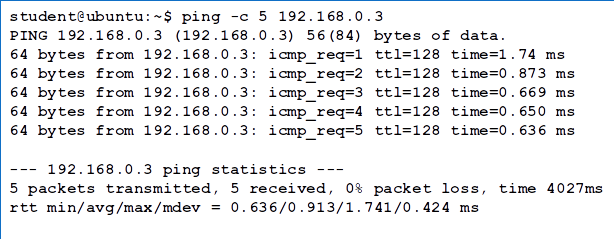
\includegraphics[width=0.8\linewidth]{ping.png}
    \end{center}
  \end{figure}
\end{frame}

\begin{frame}{Some useful network card checking commands (\texttt{18.04})}
  \begin{itemize}
    \item You need to have \texttt{ethtool} installed.
    \begin{itemize}
      \item \texttt{\$sudo apt-get install ethtool}
    \end{itemize}
    \item Card Info
    \begin{itemize}
      \item \texttt{\$sudo ethtool ens033}
      \item \texttt{\$sudo ethtool -p ens033}
    \end{itemize}
  \end{itemize}
  \begin{block}{SYNTAX}
    \begin{center}
      \texttt{ethtool [option] <network device>}
    \end{center}
  \end{block}
\end{frame}

\begin{frame}{Check your \texttt{DNS} settings.}
  \begin{itemize}
    \item \texttt{DNS} test.
    \begin{itemize}
      \item \texttt{\$nslookup www.google.com}
    \end{itemize}
    \item If \texttt{nslookup} is not found then install the \texttt{DNS} utilities package.
    \begin{itemize}
      \item \texttt{\$sudo apt-get install dnsutils}
    \end{itemize}
  \end{itemize}
\end{frame}

\begin{frame}{Check your \texttt{DNS} settings.}
  \begin{itemize}
    \item \texttt{\$nslookup www.google.com}
  \end{itemize}
  \begin{figure}
    \begin{center}
      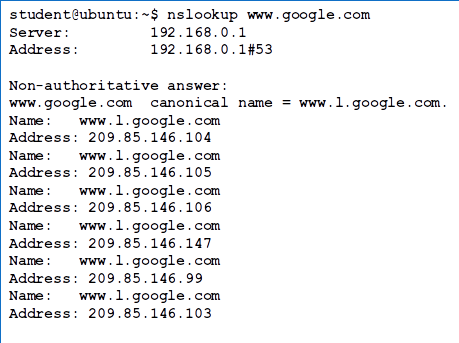
\includegraphics[width=0.8\linewidth]{nslookup.png}
    \end{center}
  \end{figure}
\end{frame}
\section*{Summary}

\begin{frame}{Summary}
  \begin{itemize}
    \item How do you install \texttt{Ubuntu Server}?
    \item What is headless mode?
    \item How do you access a headless server?
    \item How do you apply a static address?
    \begin{itemize}
      \item \texttt{IP, NETMASK, GATEWAY, DNS} (name servers)
    \end{itemize}
  \end{itemize}
\end{frame}

\end{document}


